In this chapter, the text-aware process prediction model’s performance is evaluated based on simulated and real-world event data.
First, the evaluation method and the data sets are described.
Then, the performance of differently parameterized text-aware prediction models on the data sets is analyzed in-depth and compared to two current state-of-the-art process prediction methods.

\section{Evaluation Method}

The text-aware process prediction model is evaluated on three event logs based on four prediction tasks: next activity, next timestamp, outcome, and cycle time prediction.
The text-aware model is compared to two other process prediction methods.
First, the pure LSTM approach based on the ideas of \citeauthor{DBLP:conf/caise/TaxVRD17} \cite{DBLP:conf/caise/TaxVRD17} and \citeauthor{DBLP:conf/ssci/NavarinVPS17} \cite{DBLP:conf/ssci/NavarinVPS17} is considered, which only uses the activity, timestamp, and additional non-textual attributes of each event.
This approach can be considered the state-of-the-art in process prediction if prediction performance is the only criteria.

The second baseline is the process model-based prediction method originally presented by \citeauthor{DBLP:journals/is/AalstSS11} \cite{DBLP:journals/is/AalstSS11}.
This approach constructs an annotated transition system for a log using a sequence, bag, or set abstraction.
Each state of the transition system is annotated with measurements of historical traces that can be used to predict target values for unseen traces.
During the prediction phase, running traces are mapped to the corresponding state of the transition system, and the measurements of the state are used to compute a prediction.

While the original work by \citeauthor{DBLP:journals/is/AalstSS11} focuses on regression tasks, \citeauthor{DBLP:journals/sosym/TaxTZ20} \cite{DBLP:journals/sosym/TaxTZ20} describe how an annotated transition system can also be used for classification tasks, like the next activity prediction.
For classification tasks, the measurements of each state are used to compute a probability distribution over the prediction target.
During prediction, the most likely class is predicted, given the probability distribution of the corresponding state.
For regression tasks, the mean of the measurements of each state is computed.
The eight most recent events of a trace are considered for the construction of the state space.
Experiments with different horizon lengths (1, 2, 4, 16) mostly led to worse result, so that these are not reported.

Each prediction model is evaluated with the same consistent procedure.
In the first step, the event log is separated into a training and test log. 
The training log consists of the first 2/3 chronologically ordered traces and is used to fit the prediction model to the historical event data.
The remaining 1/3 of traces are used to measure the prediction performance.
Because of the temporal dimension in event data and the potential existence of concept drifts, no cross-validation is applied.
For each trace $\sigma$ in the training and test log, all prefixes $hd^k(\sigma)$ of length $1 \leq k \leq |\sigma|$ are considered instances.

For classification (i.e., categorical prediction) task, like next event and outcome prediction, the weighted-average F$_1$ score is utilized as metric.
The F$_1$ score is a metric to measure the quality of predictors on binary classification tasks developed by \citeauthor{DBLP:books/bu/Rijsbergen79} \cite{DBLP:books/bu/Rijsbergen79}.

In a binary classification setting, instances from a data set have either a positive or negative label that needs to be predicted.
A predictor classifies each instance and separates them in four different groups:
correctly classified positive instances (true positives), incorrectly classified positive instances (false positives), correctly classified negative instances (true negatives), and incorrectly classified negative instances (false negatives).
Figure \ref{fig:/binary-classification} visualizes these four basic measures of binary classification.

Given these measures, the precision and recall of a binary classifier can be computed \cite{DBLP:journals/corr/abs-2010-16061}.
The precision of a binary classifier is the number of true positives divided by the total number of positive classified instances, i.e.,
\begin{equation*}
	\textrm{precision} = \dfrac{\textrm{true positives}}{\textrm{true positives} + \textrm{false positives}} \in [0,1].
\end{equation*}
The recall is defined as the number of true positives divided by the total number of actually positive instances, i.e.,
\begin{equation*}
	\textrm{recall} = \dfrac{\textrm{true positives}}{\textrm{true positives} + \textrm{false negatives}} \in [0,1].
\end{equation*}
The F$_1$ score combines both metrics. It is defined as the harmonic mean of precision and recall \cite{DBLP:journals/corr/abs-2010-16061}:
\begin{equation*}
	\textrm{F}_1= 2 \cdot \dfrac{\textrm{precision} \cdot \textrm{recall}}{\textrm{precision} + \textrm{recall}} = \dfrac{\textrm{true positives}}{\textrm{true positives} + \frac{1}{2} (\textrm{false positives}+\textrm{false negatives})} \in [0,1].
\end{equation*}
The precision, recall and F$_1$ score of a binary classifier can have values between 0 and 1, where 1 is the best possible value.
The F$_1$ score can be extended for multi-class classification by averaging over the one-vs.-rest F$_1$ scores per class.
The weighted-average F$_1$ score weights each class-dependent F$_1$ score with its support, i.e., the number of true instances per class.

\begin{figure}[htbp!]
	\centering
	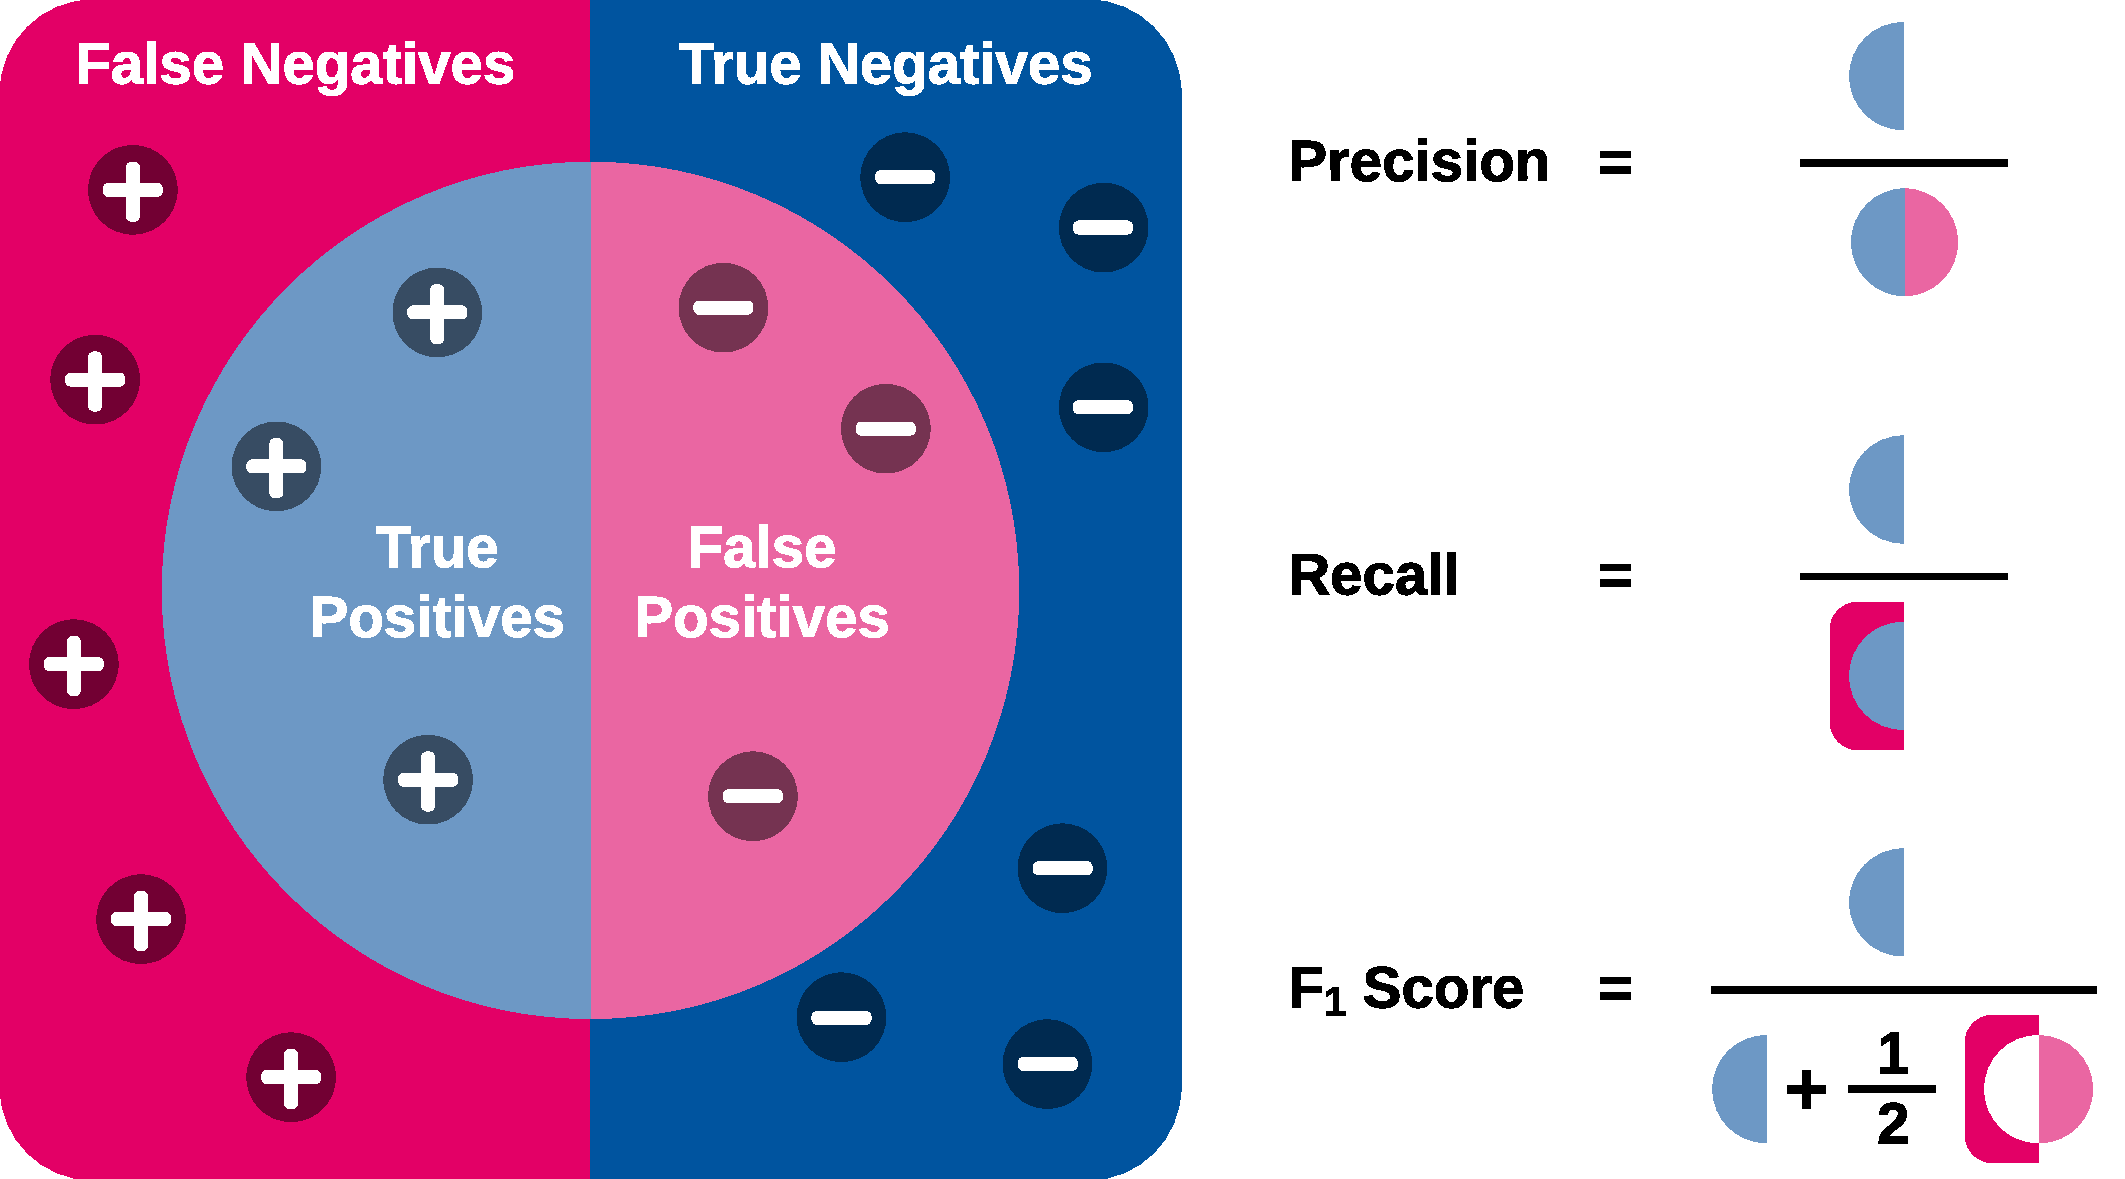
\includegraphics[width=0.75\textwidth]{figures/binary-classification}
	\caption[Visualization of binary classification and its performance measures]{Visualization of binary classification and its performance measures. Instances are either positively or negatively labeled.}
	\label{fig:/binary-classification}
\end{figure}

Let $C>2$ be the number of classes, and let $n$ be the total number of instances.
Furthermore, let F$_1^i$ be the one-vs.-rest F$_1$ score of class $i \in [C]$, and let $n_i$ be the number of instances with class $i$.
Then, the weighted-average F$_1$ score is defined as
\begin{equation*}
	\textrm{F}_1^\mathrm{weighted} = \dfrac{1}{n} \sum_{i = 1}^{C} \mathrm{F}_1^i \cdot n_i \in [0,1].
\end{equation*}
This evaluation metric is preferred over accuracy to address imbalanced distributions of target variables.
Since only multi-class prediction tasks are considered in this evaluation, F$_1$ is written to describe F$_1^\mathrm{weighted}$ in the following.

For regression tasks, like the next event time and the cycle time prediction, the mean absolute error (MAE) is computed to measure the prediction performance. The mean absolute error indicates the average absolute difference between the predicted value $\hat{y}$ and the true value $y$, i.e.,
\begin{equation*}
	\textrm{MAE} = \dfrac{1}{n}\sum_{i=1}^{n}|\hat{y_i} - y_i| \in [0, \infty).
\end{equation*}
This error metric is favored since it gives a more intuitive interpretation and is less sensitive to outliers compared to similar metrics like the mean squared error (MSE).
A MAE of 0 is the most desirable result.

The text-aware process prediction model is evaluated with all presented text models, namely the Bag of Words, Bag of N-Gram, Paragraph Vector, and Latent Dirichlet Allocation.
Each model is tested with three different encoding lengths for textual data.
The BoW and BoNG models are evaluated with 50, 100, and 500 dimensional text vectors.
The PV and LDA models are tested with smaller text encodings of size 10, 20, and 100, since they generate distributed representations.
For the BoW and BoNG model the encoding length is adjusted by only considering the most frequent terms in the vocabulary after preprocessing.
The encoding dimension of the non-textual data depends on the considered attributes and their number of the distinct values in the event logs.
The Bag of N-Gram model is used with bigrams ($n = 2$).
The Paragraph Vector model is trained for 15 epochs using a sliding window of size 8 to learn the text representations.

The LSTM network uses 100 hidden neurons per layer.
Experiments with less (75) and more (125) neurons led to slightly worse results so that these are not reported.
The network is trained with at most 25 epochs, and the learning rate is initialized with 0.001.
During the training of the LSTM model, 20\% of the training log is used for validation.
If the error on the validation log is not decreasing for two epochs in a row, the training rate is reduced by a factor of 10.
If the error does not decrease for three epochs in a row, the training is stopped in order to avoid overfitting.
Furthermore, the LSTM layers use dropout of 20\% during training as an additional measure against overfitting.


\section{Data Sets}\label{sec:datasets}

The process prediction models are evaluated on one simulated and two real-world event logs.
The three event logs describe a job application, customer journey, and hospital admission process.
Each event log contains events with textual data and is described in the following.
An overview of the key properties of the logs is summarized in Table \ref{tab:logs}.

\begin{table}[!htbp]
	\setlength\tabcolsep{5pt}
	\begin{tabularx}{\textwidth}{l c c c}
		\toprule
		\textbf{Event Log} & \textbf{Job} & \textbf{Customer} & \textbf{Hospital}  \\
		& \textbf{Application} & \textbf{Journey} &\textbf{Admission}  \\
		\midrule
		Log type & Simulated & Real-world & Real-word\\
		Cases & 20\,000& 15\,001& 46\,520\\
		Trace variants &41 & 1001 &2784 \\
		Events & 118\,811 & 55\,220 & 117\,952\\
		Events per case (mean) & 5.941& 3.681& 2.536\\
		Median case duration (days) & 1.9876 & 0.224& 7.579\\
		Mean case duration (days)& 3.1524 &  0.713 & 121.154\\
		Activities & 11 & 18 & 26\\
		Words before preprocessing & 3\,050\,594 &247\,010 &  171\,938\\
		Words after preprocessing  &1\,519\,199 &98\,915 & 165\,285\\
		Vocabulary before preprocessing & 237 & 1203 & 4973 \\
		Vocabulary after preprocessing & 185 & 817 & 4633\\
		Text attribute & Email& Customer question & Diagnosis\\
		Additional non-textual attributes & - & Gender& Admission type\\
		&  & Age& Insurance\\
		\bottomrule
	\end{tabularx}
	\caption[Overview of the evaluated event logs]{Overview of the evaluated event logs with their key properties.}
	\label{tab:logs}
\end{table}

\textbf{Job Application} (simulated log) This event log describes a simple job application process. 
First, the applicant starts an application in the company’s system.
The candidate then uploads a curriculum vitae (CV) and optionally a cover letter in random order.
When the documents have been received, the applicant is either directly rejected by the company or invited to an interview.
In case of an invitation, the applicant responds with an acceptance or rejection email.
After the interview, a decision is made and sent to the applicant that states whether the applicant gets a job offer or is rejected.
In case of a job offer, the applicant answers again with an acceptance or rejection email.
In total, the process contains up to 5 text documents (CV, cover letter, accept/reject interview email by the candidate, job offer/reject email by the company, and accept/reject job offer email by the candidate).

The timestamp of each event is determined by sampling from a normal distribution, which mean and variance is unique per activity.
The CV, cover letter, and all emails are available as a text attribute in the event log.
The text information is generated by sampling 10 times from sets of full and partial sentences depending on the control flow of the process instance.
For example, if an applicant gets a job offer, the generated email contains text fragments from typical job offer emails.
If the applicant is rejected, the email is generated with sentences from typical rejection emails instead.
With this text generation mechanism, all texts in the event log are unique, but the words and sentences in the texts correlate with the path of the corresponding case.
Furthermore, noise is added by introducing a 1\% probability after each event that the process stops immediately and is not finished properly.
A model of the simulated process is shown in Figure \ref{fig:/application-process} using BPMN \cite{BPMN} notation.

\begin{figure}[htbp!]
	\centering
	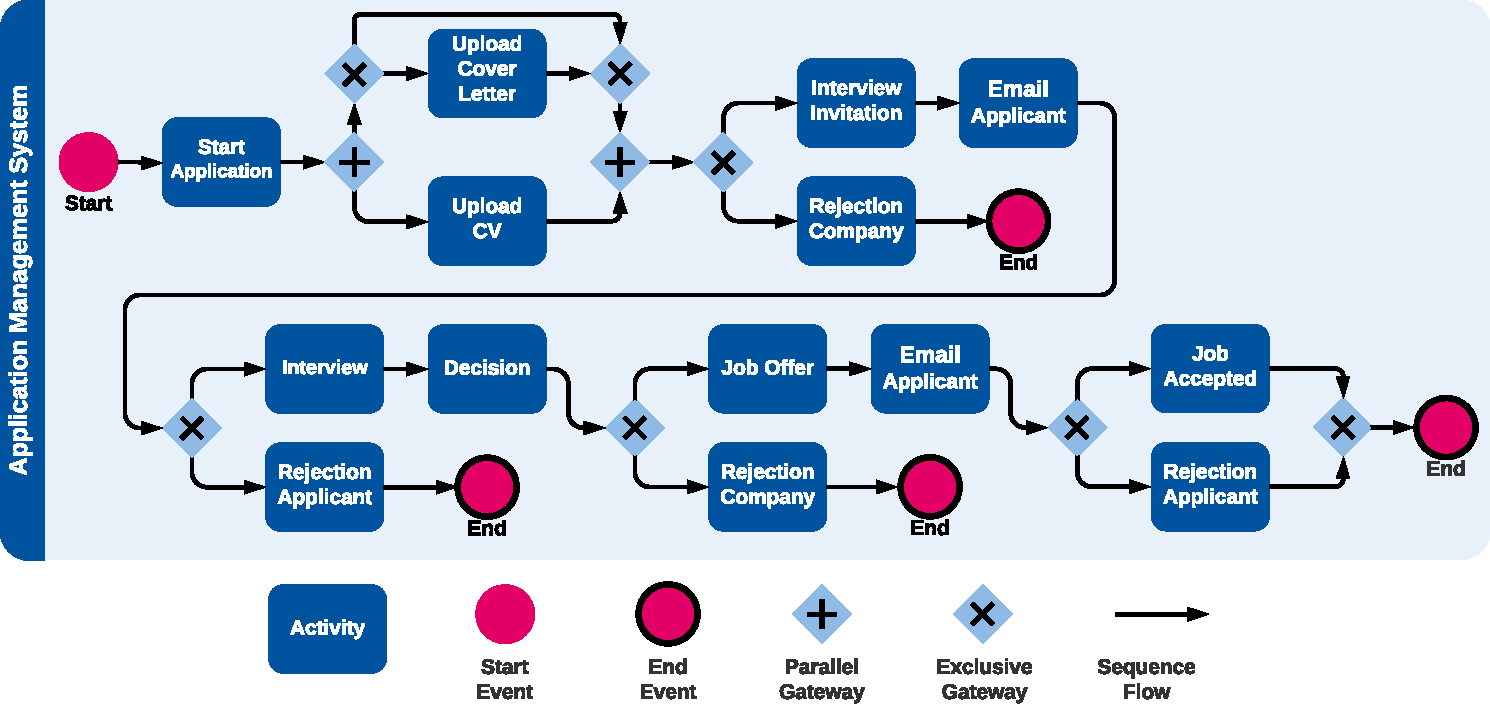
\includegraphics[width=\textwidth]{figures/application-process}
	\caption[BPMN model of the job application process]{BPMN model of the job application process. For simplicity, only the performed activities and the control flow are modeled. An enlarged version of this figure is provided in Appendix \ref{appendix-a}.}
	\label{fig:/application-process}
\end{figure}

\textbf{Customer Journey} (real-world log) This event log describes customer's journeys of the Employee Insurance Agency commissioned by the Dutch Ministry of Social Affairs and Employment.
The log is aggregated from two anonymized data sets provided in the BPI Challenge 2016 \cite{bpichallenge2016}, containing click data of customers logged in the official website werk.nl and phone call data from their call center.
Both data sets are joined based on the customer ID to derive a detailed view of customer contacts on the web and the phone.
For each phone call, the customer’s question is available as a text attribute in English.
Click events on the website do not contain any textual data.
In addition, the customer’s age (grouped) and gender are considered as additional attributes.
The event log is filtered to remove outlier activities (threshold <0.5\%) and infrequent trace variants (2 or fewer traces with the same variant).

\textbf{Hospital Admission} (real-world log) This log is generated from the MIMIC-III (Medical Information Mart for Intensive Care) database \cite{johnson2016mimic} and contains hospital admission and discharge events of patients in the Beth Israel Deaconess Medical Center between 2001 and 2012.
Next to the admission and discharge locations that define the activity, the admission type (e.g., emergency) and insurance (e.g., private) of the patient are considered as additional attributes.
Furthermore, each admission event contains a short diagnosis as a text attribute.
A case contains all the admission and discharge events of a single patient.
Admission and discharge events occur alternating, so that every admission event is followed by a discharge event.

All three logs represent different levels of process complexity and variability.
The job application log is the most structured log containing 11 different activities, 41 trace variants, and a vocabulary of 185 unique words after preprocessing.
Therefore, this log can be considered as quite simple and is subsequently easier to predict.
In contrast, the customer journey log has 18 different activities, 1001 trace variants, and 817 unique words.
The hospital admission log is the most complex with 26 activities, 2784 trace variants, and 4633 unique words.
Short snippets of all three event logs with the considered data attributes are provided in Appendix \ref{appendix-b}.

\section{Next Activity and Timestamp Prediction}

First, the prediction performance regarding the next event's activity and timestamp is evaluated for all prefix traces in the test log.
The results are summarized in Table \ref{tab:next-event}.
Each line in the table states the F$_1$ score for the next activity and the mean absolute error in days for the next timestamp prediction of a single model on each evaluated event log.

\begin{table}[!htbp]
	\newrobustcmd{\B}{\fontseries{b}\selectfont}
	\setlength\tabcolsep{2pt}
	\begin{tabularx}{\textwidth}{
			>{\hsize=0.8\hsize}C
			>{\hsize=1.2\hsize}C
			>{\hsize=1.0\hsize}C
			>{\hsize=1.0\hsize}C
			>{\hsize=1.0\hsize}C
			>{\hsize=1.0\hsize}C
			>{\hsize=1.0\hsize}C
			>{\hsize=1.0\hsize}C
		}
		\toprule
		& & \multicolumn{2}{l}{\textbf{Job Application}} & \multicolumn{2}{l}{\textbf{Customer Journey}} & \multicolumn{2}{l}{\textbf{Hospital Admission}} \\
		Text & Text &Activity & Time & Activity& Time  & Activity& Time  \\
		Model & Vector Size &F$_1$ Score & MAE (days) & F$_1$ Score& MAE (days)  & F$_1$ Score& MAE (days)  \\
		\midrule
		\multicolumn{8}{c}{\textit{Text-Aware Process Prediction (LSTM + Text Model)}} \\
BoW&50&     0.8549&     0.1037&     0.4251&     0.1764&     0.5389&    29.0819  \\
BoW&100&     0.8806&     0.1053&     0.4304&  \B   0.1763&     0.5487&    31.4378 \\
BoW&500&     0.8550&     0.1037&  \B   0.4312&     0.1798& \B    0.5596&    27.5495 \\
BoNG&50&     0.8386&     0.1335&     0.4270&     0.1767&     0.5309&    27.5397 \\
BoNG&100&     0.8803&     0.1088&     0.4237&     0.1770&     0.5450&    28.3293 \\
BoNG&500&     0.8629&     0.1053&     0.4272&     0.1773&     0.5503&    27.9720 \\
PV&10&     0.7988&     0.1814&     0.4112&     0.1812&     0.5265&    29.4610 \\
PV&20&     0.8451&     0.1175&     0.4134&     0.1785&     0.5239&  \B  27.2902 \\
PV&100&     0.8619&     0.1162&     0.4162&     0.1789&     0.5292&    28.2369 \\
LDA&10&     0.8547&     0.1033&     0.4239&     0.1786&     0.5252&    28.8553 \\
LDA&20&     0.8583&     0.1039&     0.4168&     0.1767&     0.5348&    27.8830 \\
LDA&100&  \B   0.8830&  \B   0.1032&     0.4264&     0.1777&     0.5418&    27.5084 \\
		\multicolumn{8}{c}{\textit{LSTM Model Prediction Baseline}}  \\
\multicolumn{2}{l}{LSTM \cite{DBLP:conf/caise/TaxVRD17}+\cite{DBLP:conf/ssci/NavarinVPS17}} & 0.6987&     0.2499&     0.4029&     0.1781&     0.5187&    27.7571\\
		\multicolumn{8}{c}{\textit{Process Model Prediction Baseline (Annotated Transition System)}} \\
\multicolumn{2}{l}{Sequence \cite{DBLP:journals/is/AalstSS11}+\cite{DBLP:journals/sosym/TaxTZ20}}&   0.7239&     0.2553&     0.4005&     0.2387&     0.4657&    64.0161\\
\multicolumn{2}{l}{Bag \cite{DBLP:journals/is/AalstSS11}+\cite{DBLP:journals/sosym/TaxTZ20}} &   0.7159&     0.2553&     0.3634&     0.2389&     0.4681&    64.6567\\
\multicolumn{2}{l}{Set \cite{DBLP:journals/is/AalstSS11}+\cite{DBLP:journals/sosym/TaxTZ20}} &     0.7065&     0.2553&     0.3565&     0.2389&     0.4397&    63.2042\\
		\bottomrule
	\end{tabularx}
	\caption[Experimental results for the next activity and timestamp prediction]{Experimental results for the next activity and timestamp prediction.}
	\label{tab:next-event}
\end{table}

Compared to the baseline approaches, the text-aware model can improve the next activity and timestamp prediction on all data sets with at least one parameterization.
Markedly, the impact of the consideration of textual data varies a lot between the data sets and the prediction tasks.
A reason for that might be that the textual data in the simulated log clearly correlates with the control flow by design, where, in the real-world event logs, the correlation is only assumed and probably significantly lower.

On the job application log, the F$_1$ score of the next activity prediction goes up to 0.8830 using the LDA text model.
This is an improvement of 0.1843 compared to the LSTM baseline.
The next timestamp prediction is improved by up to 0.1467 days (around 3.5 hours).
The other encoding models perform similarly with the exception of the PV model in combination with a small 10 dimensional text encoding.
Since this log contains rather long text documents, the small encoding size is not able to represent the textual data sufficiently.
The process model baselines using the annotated transition system perform similarly to the LSTM baseline approach but significantly worse than the text-aware approaches.
The transition system created using a sequence abstraction performs slightly better than the other baselines.
Nevertheless, the trace abstraction method has a rather small impact on the prediction quality.

In contrast, on the customer journey log, the next activity F$_1$ score is improved by at most 0.0283 using the BoW model compared to the LSTM baseline.
The impact of the text-awareness on next timestamp prediction is negligible on this log.
Seven out of the twelve text-aware models improve the next timestamp prediction, while five are slightly worse.
The annotated transition system generates slightly worse next activity and timestamps predictions.
Again, the sequence abstraction outperforms the other trace abstractions.

The F$_1$ score is improved on the hospital admission log by up to 0.0409 using the BoW model and a 500 dimensional text encoding compared to the LSTM baseline.
It can be observed that on this log, the high dimensional encodings tend to perform better.
This probably comes down to the fact that the hospital log with 4\,633 unique words has the largest vocabulary by far, and therefore larger text encodings are required.
Regarding the next timestamp prediction, the PV model with 20 dimensional text vectors performs the best.
However, the positive impact of the textual data is questionable since some text models also perform worse, like the BoW model with 100 dimensional text encoding.
The process model baselines fall back clearly on both prediction tasks on the hospital admission log.
It is assumed that the huge amount of trace variants on this log is disadvantageous for prediction models with a discrete set of states.
In contrast, the LSTM models can profit from their noise resistance.

The choice of text model has a rather small impact on the results on all event logs.
Notably, the BoW and LDA model perform most consistently on all data sets and all text encoding lengths.
The PV model reaches slightly worse results, especially when a small text embedding size is used.
The BoNG model has a similar performance compared to the BoW model.
Surprisingly, the word order awareness of the BoNG model does not lead to better prediction results in general.

\definecolor{bow}{RGB}{227,0,102}
\definecolor{bong}{RGB}{233,96,136}
\definecolor{pv}{RGB}{241,158,177}
\definecolor{lda}{RGB}{249,210,218}

\definecolor{lstm}{RGB}{100,100,100}

\definecolor{sequence}{RGB}{0,84,159}
\definecolor{bag}{RGB}{64,127,183}
\definecolor{set}{RGB}{142,186,229}

\pgfplotscreateplotcyclelist{colorlist}{%
	bow,line width=0.7pt,every mark/.append style={line width=160pt, fill=bow,},mark=o, mark options={scale=1.6}\\%1
	bong,line width=0.7pt,every mark/.append style={fill=bong},mark=diamond, mark options={scale=1.8}\\%2
	pv,line width=0.7pt,every mark/.append style={fill=pv},mark=otimes, mark options={scale=1.4}\\%3
	lda,line width=0.7pt,every mark/.append style={fill=lda},mark=star, mark options={scale=1.6}\\%4
	lstm,line width=0.7pt,every mark/.append style={fill=lstm},mark=square, mark options={scale=1.6}\\%5
	sequence,line width=0.7pt, every mark/.append style={fill=sequence},mark=10-pointed star, mark options={scale=1.2}\\%6
	bag,line width=0.7pt,every mark/.append style={fill=bag},mark=triangle, mark options={scale=1.8}\\%7
	set,line width=0.7pt,every mark/.append style={fill=set},mark=oplus, mark options={scale=1.3}\\%8
}

\begin{figure}[!htbp]
	\centering
	\begin{subfigure}{\textwidth}
		\centering
		\begin{tikzpicture} 
			\begin{axis}[
				scale only axis,width=1mm, height=1mm,
				hide axis,
				draw=none,
				legend columns=-1,
				legend style={/tikz/every even column/.append style={column sep=0.2cm}, draw=none},
				cycle list name = colorlist,
				legend style={at={(10,5)}},
				legend image post style={sharp plot},
				]
				\pgfplotsinvokeforeach{1,...,8}{\addplot coordinates {(0,0)};} 
				\addlegendentry{BoW};
				\addlegendentry{BoNG};
				\addlegendentry{PV};
				\addlegendentry{LDA};
				\addlegendentry{LSTM};
				\addlegendentry{Sequence};
				\addlegendentry{Bag};
				\addlegendentry{Set};
			\end{axis}
		\end{tikzpicture}%
		\vfill
		\vspace{0.3cm}
		\begin{tikzpicture}[scale=0.9]
			\begin{axis}[
				xlabel={Prefix Length},
				ylabel={F$_1$ Score},
				cycle list name=colorlist,
				]	
				\addplot table[x=index,y=naBoW100, col sep= comma] {data/prefix_application.csv};
				\addlegendentry{BoW}
				\addplot table[x=index,y=naBoNG100, col sep= comma]  {data/prefix_application.csv};
				\addlegendentry{BoNG}
				\addplot table[x=index,y=naPV100, col sep= comma]  {data/prefix_application.csv};
				\addlegendentry{PV}
				\addplot table[x=index,y=naLDA100, col sep= comma] {data/prefix_application.csv};
				\addlegendentry{LDA}
				\addplot table[x=index,y=na-0, col sep= comma] {data/prefix_application.csv};
				\addlegendentry{LSTM}
				\addplot table[x=index,y=nasequence8, col sep= comma] {data/prefix_application.csv};
				\addlegendentry{Sequence}
				\addplot table[x=index,y=nabag8, col sep= comma] {data/prefix_application.csv};
				\addlegendentry{Bag}
				\addplot table[x=index,y=naset8, col sep= comma] {data/prefix_application.csv};
				\addlegendentry{Set}
				\legend{}
			\end{axis}
		\end{tikzpicture}%
		\hfill
		\begin{tikzpicture}[scale=0.9]
			\begin{axis}[
				xlabel={Prefix Length},
				ylabel={Mean Absolute Error (days)},
				cycle list name=colorlist,
				]
				\addplot table[x=index,y=ntBoW500, col sep= comma] {data/prefix_application.csv};
				\addlegendentry{BoW}
				\addplot table[x=index,y=ntBoNG500, col sep= comma]  {data/prefix_application.csv};
				\addlegendentry{BoNG}
				\addplot table[x=index,y=ntPV100, col sep= comma]  {data/prefix_application.csv};
				\addlegendentry{PV}
				\addplot table[x=index,y=ntLDA100, col sep= comma] {data/prefix_application.csv};
				\addlegendentry{LDA}
				\addplot table[x=index,y=nt-0, col sep= comma] {data/prefix_application.csv};
				\addlegendentry{LSTM}
				\addplot table[x=index,y=ntsequence8, col sep= comma] {data/prefix_application.csv};
				\addlegendentry{Sequence}
				\addplot table[x=index,y=ntbag8, col sep= comma] {data/prefix_application.csv};
				\addlegendentry{Bag}
				\addplot table[x=index,y=ntset8, col sep= comma] {data/prefix_application.csv};
				\addlegendentry{Set}
				\legend{}
			\end{axis}
		\end{tikzpicture}
		\caption{Job application event log.}
		\vspace{0.3cm}
	\end{subfigure}
	\begin{subfigure}{\textwidth}
		\centering
		\begin{tikzpicture}[scale=0.9, spy using outlines={circle, magnification=1.0,connect spies, lens={scale=1.9}} ]
			\begin{axis}[
				xlabel={Prefix Length},
				ylabel={F$_1$ Score},
				cycle list name=colorlist,
				]
				\addplot table[x=index,y=naBoW500, col sep= comma] {data/prefix_werk.csv};
				\addlegendentry{BoW}
				\addplot table[x=index,y=naBoNG500, col sep= comma] {data/prefix_werk.csv};
				\addlegendentry{BoNG}
				\addplot table[x=index,y=naPV100, col sep= comma]  {data/prefix_werk.csv};
				\addlegendentry{PV}
				\addplot table[x=index,y=naLDA100, col sep= comma] {data/prefix_werk.csv};
				\addlegendentry{LDA}
				\addplot table[x=index,y=na-0, col sep= comma] {data/prefix_werk.csv};
				\addlegendentry{LSTM}
				\addplot table[x=index,y=nasequence8, col sep= comma] {data/prefix_werk.csv};
				\addlegendentry{Sequence}
				\addplot table[x=index,y=nabag8, col sep= comma] {data/prefix_werk.csv};
				\addlegendentry{Bag}
				\addplot table[x=index,y=naset8, col sep= comma] {data/prefix_werk.csv};
				\addlegendentry{Set}
				\coordinate (spypoint) at (axis cs:1.3,0.245);
				\coordinate (spyviewer) at (axis cs:2.1,0.71);
				\spy[width=2.7cm,height=2.7cm] on (spypoint) in node [fill=white] at (spyviewer);
				\coordinate (spypoint2) at (axis cs:5.7,0.73);
				\coordinate (spyviewer2) at (axis cs:5.7,0.35);
				\spy[width=2.7cm,height=2.7cm] on (spypoint2) in node [fill=white] at (spyviewer2);
				\legend{}
			\end{axis}
		\end{tikzpicture}%
		\hfill
		\begin{tikzpicture}[scale=0.9, spy using outlines={circle, magnification=1.0,connect spies, lens={scale=1.8},}]
			\begin{axis}[
				xlabel={Prefix Length},
				ylabel={Mean Absolute Error (days)},
				cycle list name=colorlist,
				]
				\addplot table[x=index,y=ntBoW100, col sep= comma] {data/prefix_werk.csv};
				\addlegendentry{BoW}
				\addplot table[x=index,y=ntBoNG50, col sep= comma] {data/prefix_werk.csv};
				\addlegendentry{BoNG}
				\addplot table[x=index,y=ntPV20, col sep= comma]  {data/prefix_werk.csv};
				\addlegendentry{PV}
				\addplot table[x=index,y=ntLDA20, col sep= comma] {data/prefix_werk.csv};
				\addlegendentry{LDA}
				\addplot table[x=index,y=nt-0, col sep= comma] {data/prefix_werk.csv};
				\addlegendentry{LSTM}
				\addplot table[x=index,y=ntsequence8, col sep= comma] {data/prefix_werk.csv};
				\addlegendentry{Sequence}
				\addplot table[x=index,y=ntbag8, col sep= comma] {data/prefix_werk.csv};
				\addlegendentry{Bag}
				\addplot table[x=index,y=ntset8, col sep= comma] {data/prefix_werk.csv};
				\addlegendentry{Set}
				\coordinate (spypoint) at (axis cs:2.10,0.095);
				\coordinate (spyviewer) at (axis cs:5.0,0.3);
				\spy[width=3.0cm,height=3.0cm] on (spypoint) in node [fill=white] at (spyviewer);
				\legend{}
			\end{axis}
		\end{tikzpicture}
		\caption{Customer journey event log.}
		\vspace{0.3cm}
	\end{subfigure}
	\begin{subfigure}{\textwidth}
		\centering
		\begin{tikzpicture}[scale=0.9, spy using outlines={circle, magnification=1.0,connect spies, lens={scale=2},}]
			\begin{axis}[
				xlabel={Prefix Length},
				ylabel={F$_1$ Score},
				cycle list name=colorlist,
				]
				\addplot table[x=index,y=naBoW500, col sep= comma] {data/prefix_admissions.csv};
				\addlegendentry{BoW}
				\addplot table[x=index,y=naBoNG500, col sep= comma] {data/prefix_admissions.csv};
				\addlegendentry{BoNG}
				\addplot table[x=index,y=naPV100, col sep= comma]  {data/prefix_admissions.csv};
				\addlegendentry{PV}
				\addplot table[x=index,y=naLDA100, col sep= comma] {data/prefix_admissions.csv};
				\addlegendentry{LDA}
				\addplot table[x=index,y=na-0, col sep= comma] {data/prefix_admissions.csv};
				\addlegendentry{LSTM}
				\addplot table[x=index,y=nasequence8, col sep= comma] {data/prefix_admissions.csv};
				\addlegendentry{Sequence}
				\addplot table[x=index,y=nabag8, col sep= comma] {data/prefix_admissions.csv};
				\addlegendentry{Bag}
				\addplot table[x=index,y=naset8, col sep= comma] {data/prefix_admissions.csv};
				\addlegendentry{Set}
				\coordinate (spypoint) at (axis cs:2.53,0.3);
				\coordinate (spyviewer) at (axis cs:6.4,0.61);
				\spy[width=2cm,height=2cm] on (spypoint) in node [fill=white] at (spyviewer);
				\legend{}
			\end{axis}
		\end{tikzpicture}%
		\hfill
		\begin{tikzpicture}[scale=0.90]
			\begin{axis}[
				xlabel={Prefix Length},
				ylabel={Mean Absolute Error (days)},
				cycle list name=colorlist,
				]
				\addplot table[x=index,y=ntBoW500, col sep= comma] {data/prefix_admissions.csv};
				\addlegendentry{BoW}
				\addplot table[x=index,y=ntBoNG50, col sep= comma] {data/prefix_admissions.csv};
				\addlegendentry{BoNG}
				\addplot table[x=index,y=ntPV20, col sep= comma]  {data/prefix_admissions.csv};
				\addlegendentry{PV}
				\addplot table[x=index,y=ntLDA100, col sep= comma] {data/prefix_admissions.csv};
				\addlegendentry{LDA}
				\addplot table[x=index,y=nt-0, col sep= comma] {data/prefix_admissions.csv};
				\addlegendentry{LSTM}
				\addplot table[x=index,y=ntsequence8, col sep= comma] {data/prefix_admissions.csv};
				\addlegendentry{Sequence}
				\addplot table[x=index,y=ntbag8, col sep= comma] {data/prefix_admissions.csv};
				\addlegendentry{Bag}
				\addplot table[x=index,y=ntset8, col sep= comma] {data/prefix_admissions.csv};
				\addlegendentry{Set}
				\legend{}
			\end{axis}
		\end{tikzpicture}
		\caption{Hospital admission event log.}
	\end{subfigure}
	\caption[Next activity and timestamp prediction performance depending on the prefix length]{Next activity (left) and timestamp (right) prediction performance depending on the prefix length for each evaluated event log.}
	\label{fig:next-activity-prefix}
\end{figure}

In addition, the prediction performance is reported per prefix length for each event log.
Figure \ref{fig:next-activity-prefix} shows the F$_1$ score and next timestamp MAE for every prefix trace of length $1 \leq k \leq 8$.
Please note that the results on shorter traces are supported by a much larger set of traces due to prefix generation during the construction of the training and test data sets.
For the text-aware models, only the best text encoding length is shown in the diagram.

On the job application event log, all text-aware process models almost perfectly predict the next activity after three events (i.e., after the application documents are available).
The baseline approaches cannot take advantage of the emails and reaches an F$_1$ score of around 0.75 after the first three events.
This shows that all text-aware approaches can unequivocally take advantage of the textual data at every decision point in the process, despite the fact that all documents in the log are unique.
The improvements in the activity prediction lead consequently to significantly better timestamp predictions on this log.

On the customer journey log, the prediction performance of all models correlates positively with the available prefix length of the trace.
The next activity F$_1$ score is improved from under 0.3, when only the first event is available, to over 0.8 after eight events for all models.
All text-aware prediction models surpass the baseline approaches on very short prefix traces of length 3 or shorter.
There are two possible explanations for this.
First, the events holding textual data seem to appear mostly at the beginning of the traces in this log.
Furthermore, in order to generalize from the textual data, usually, more training data is necessary.
Since there are always more short prefixes available in the training set, the text-aware models benefit disproportionately on shorter traces.
The transition system created using a sequence abstraction underperforms on shorter prefixes but outperforms all LSTM approaches on longer prefixes.
The MAE on the next timestamp prediction rapidly drops when more events are available independent of the prediction model.
The LSTM-based models have a slight advantage over the process model baseline on short prefixes.
However, no difference between text-aware models and the LSTM baseline is recognizable on this prediction task.

The hospital admission log is characterized by the alternation of admission and discharge events.
Therefore, the prediction accuracy varies between odd and even prefix lengths.
The text-aware prediction models generate slightly better predictions on admission events since only these contain the diagnosis as text attribute, which can be utilized by the text-aware models.
The prediction performance of the LSTM models on admission events is slightly increased with longer prefixes, while the accuracy on discharge events decreases.
Regarding the next timestamp prediction, higher errors after discharge events and very low errors after admission events are observed.
This can be explained by the rather short hospital stays compared to longer time periods between two hospitalizations.

\section{Outcome and Cycle Time Prediction}

The outcome and cycle time prediction are evaluated analogously to the next activity and timestamp prediction.
In contrast to the next event prediction, the target values are case properties, i.e., they are the same for every prefix trace of a case.
As an outcome, the final activity of the trace is predicted as described in Section \ref{sec:overview}.
The MAE of the cycle time prediction is measured in days.
The results of all evaluated prediction models are summarized in Table \ref{tab:outcome-cycle-time}.

\begin{table}[!htbp]
	\newrobustcmd{\B}{\fontseries{b}\selectfont}
	\setlength\tabcolsep{3pt}
	\begin{tabularx}{\textwidth}{
			>{\hsize=0.8\hsize}C
			>{\hsize=1.2\hsize}C
			>{\hsize=1.0\hsize}C
			>{\hsize=1.0\hsize}C
			>{\hsize=1.0\hsize}C
			>{\hsize=1.0\hsize}C
			>{\hsize=1.0\hsize}C
			>{\hsize=1.0\hsize}C
		}
		\toprule
		& & \multicolumn{2}{c}{\textbf{Job Application}} & \multicolumn{2}{c}{\textbf{Customer Journey}} & \multicolumn{2}{c}{\textbf{Hospital Admission}} \\
		Text & Text &Outcome & Cycle & Outcome& Cycle  & Outcome& Cycle  \\
		Model & Vector Size &F$_1$ Score & MAE (days) & F$_1$ Score& MAE (days) & F$_1$ Score& MAE (days) \\
		\midrule
		\multicolumn{8}{c}{\textit{Text-Aware Process Prediction (LSTM + Text Model)}} \\
BoW&50&     0.6516&   \B  1.3615&     0.4732&     0.2357&     0.6120&    69.2953 \\
BoW&100&     0.6523&     1.3642&     0.4690&  \B   0.2337&   \B  0.6187&    70.9488 \\
BoW&500&  \B   0.6535&     1.3678&     0.4690&     0.2354&     0.6050&    70.1084 \\
BoNG&50&     0.6449&     1.4003&     0.4789&     0.2365&     0.6099&    69.4456 \\
BoNG&100&     0.6509&     1.3700&     0.4819&     0.2373&     0.6094&    69.3619 \\
BoNG&500&     0.6492&     1.3670&     0.4692&     0.2358&     0.6052&    70.6906 \\
PV&10&     0.5935&     1.5122&     0.4670&     0.2424&     0.6007&    73.5219 \\
PV&20&     0.6401&     1.3917&     0.4732&     0.2417&     0.5962&    69.6191 \\
PV&100&     0.6464&     1.3855&     0.4707&     0.2416&     0.6058&    69.4793 \\
LDA&10&     0.6421&     1.3622&     0.4755&     0.2394&     0.6017&  \B  69.1465 \\
LDA&20&     0.6530&     1.3620&     0.4747&     0.2375&     0.6071&    69.6269 \\
LDA&100&     0.6504&     1.3662&   \B  0.4825&     0.2374&     0.6106&    69.3189 \\
		\multicolumn{8}{c}{\textit{LSTM Model Prediction Baseline}}  \\
\multicolumn{2}{l}{LSTM \cite{DBLP:conf/caise/TaxVRD17}+\cite{DBLP:conf/ssci/NavarinVPS17}} & 0.5296&     1.6765&     0.4673&     0.2455&     0.5976&    70.2978 \\
		\multicolumn{8}{c}{\textit{Process Model Prediction Baseline (Annotated Transition System)}} \\
\multicolumn{2}{l}{Sequence \cite{DBLP:journals/is/AalstSS11}+\cite{DBLP:journals/sosym/TaxTZ20}}&    0.5551&     1.8067&     0.4669&     0.2799&     0.5479&   171.5684\\
\multicolumn{2}{l}{Bag \cite{DBLP:journals/is/AalstSS11}+\cite{DBLP:journals/sosym/TaxTZ20}}&    0.5544&     1.8066&     0.4394&     0.2797&     0.5451&   173.7963\\
\multicolumn{2}{l}{Set \cite{DBLP:journals/is/AalstSS11}+\cite{DBLP:journals/sosym/TaxTZ20}}&   0.5544&     1.8069&     0.4381&     0.2796&     0.5588&   171.4487\\
		\bottomrule
	\end{tabularx}
	\caption[Experimental results for the outcome and cycle time prediction]{Experimental results for the outcome and cycle time prediction.}
	\label{tab:outcome-cycle-time}
\end{table}

On the job application log, the text-aware prediction model can predict the outcome of the case with an F$_1$ score of up to 0.6535 using the BoW text model compared to 0.5296 using the LSTM baseline approach.
Therefore, the prediction can be improved by up to 0.1239.
Other text models perform similar to the BoW model except for the PV model with 10 dimensional text vectors with an F$_1$ score of only 0.5935.
The MAE on the cycle time prediction can be reduced to 1.3615 days with the BoW model compared to 1.6765 days on the LSTM baseline approach.
The annotated transition system achieves an F$_1$ score of up 0.5551 and a cycle time MAE of 1.8066 days.

On the customer journey log, the text-awareness leads to much smaller improvements as observed for the next event prediction.
The best outcome prediction is realized with the LDA text model resulting in an F$_1$ score of 0.4825.
The cycle time MAE using the BoW model is 0.2337 days, which improves the LSTM baseline prediction by 0.0118 days (= 16.99 minutes).
All text-aware models outperform the LSTM baseline by a small amount on the cycle time prediction.
The sequence-abstracted transition system predicts the outcome with an F$_1$ score of 0.4669 and hence stays in line with the LSTM-based models.
The bag- and set-abstracted models fall back slightly.
The cycle time MAE of the annotated transition systems is at least 0.0341 days (= 49 minutes) worse compared to the LSTM-based approaches.

On the hospital admission log, the text-aware approach delivers an F$_1$ score of 0.6187 on the outcome prediction task using the BoW model.
This improves the LSTM baseline's F$_1$ score by 0.0211.
However, the cycle time prediction error is around 70 days for all LSTM-based approaches.
Nine text-aware models perform better than the LSTM baseline, the other three perform slightly worse.
As observed during the next timestamp prediction, the text-aware models have difficulties to clearly improve the performance on time-related regression tasks on this particular log.
The transition systems predict the outcome with an F$_1$ score of up to 0.5588 and have a much larger error on the cycle time prediction of at least 171.4487 days using the set abstraction.
The other abstraction methods perform noticeably worse.
Since the log contains many trace variants, the stronger set abstraction has an advantage.
Nevertheless, the extreme variability in the log creates difficulties for the process model-based approaches.
Furthermore, the unevenly distributed cycle times of the processes might be disadvantageous for the transition systems.

Again, the choice of text model has a rather small impact.
The BoW and LDA models perform slightly better than the BoNG and PV model.
Strikingly, the best predictions have always been generated by a text-aware model using either the BoW or the LDA text model.
Compared to the next activity and timestamp prediction, the improvement through the text-awareness is smaller on the case-based prediction tasks.

In addition, the prediction results are computed depending on the prefix length of the traces.
Figure \ref{fig:outcome-cycle-time-prefix} depicts the outcome F$_1$ scores and cycle time MAE per prefix on every event log and approach.
On the job application log, the F$_1$ score is improved with longer prefixes from under 0.3 after the first event to over 0.8 after eight events using any text-aware prediction model.
The F$_1$ score of the baseline approaches peaks after five events but always stays below 0.7.
The biggest quality improvements of the outcome prediction can be realized within the first three events.
The MAE on the cycle time prediction is reduced with every event on all models consistently by around 0.4 days per event.
Nevertheless, the text-aware models are able to make similar good predictions two events before the baseline models.
This shows that the text-aware approach can improve the earliness of the prediction.

\begin{figure}[!htbp]
	\centering
	\begin{subfigure}{\textwidth}
		\centering
		\begin{tikzpicture} 
			\begin{axis}[
				scale only axis,width=1mm, height=1mm,
				hide axis,
				draw=none,
				legend columns=-1,
				legend style={/tikz/every even column/.append style={column sep=0.2cm}, draw=none},
				cycle list name = colorlist,
				legend style={at={(10,5)}},
				legend image post style={sharp plot},
				]
				\pgfplotsinvokeforeach{1,...,8}{\addplot coordinates {(0,0)};} 
				\addlegendentry{BoW};
				\addlegendentry{BoNG};
				\addlegendentry{PV};
				\addlegendentry{LDA};
				\addlegendentry{LSTM};
				\addlegendentry{Sequence};
				\addlegendentry{Bag};
				\addlegendentry{Set};
			\end{axis}
		\end{tikzpicture}%
		\vfill
		\vspace{0.3cm}
		\begin{tikzpicture}[scale=0.9]
			\begin{axis}[
				xlabel={Prefix Length},
				ylabel={F$_1$ Score},
				cycle list name=colorlist,
				]			
				\addplot table[x=index,y=oaBoW500, col sep= comma] {data/prefix_application.csv};
				\addlegendentry{BoW}
				\addplot table[x=index,y=oaBoNG100, col sep= comma]  {data/prefix_application.csv};
				\addlegendentry{BoNG}
				\addplot table[x=index,y=oaPV100, col sep= comma]  {data/prefix_application.csv};
				\addlegendentry{PV}
				\addplot table[x=index,y=oaLDA20, col sep= comma] {data/prefix_application.csv};
				\addlegendentry{LDA}
				\addplot table[x=index,y=oa-0, col sep= comma] {data/prefix_application.csv};
				\addlegendentry{LSTM}
				\addplot table[x=index,y=oasequence8, col sep= comma] {data/prefix_application.csv};
				\addlegendentry{Sequence}
				\addplot table[x=index,y=oabag8, col sep= comma] {data/prefix_application.csv};
				\addlegendentry{Bag}
				\addplot table[x=index,y=oaset8, col sep= comma] {data/prefix_application.csv};
				\addlegendentry{Set}
				\legend{}
			\end{axis}
		\end{tikzpicture}%
		\hfill
		\begin{tikzpicture}[scale=0.9]
			\begin{axis}[
				xlabel={Prefix Length},
				ylabel={Mean Absolute Error (days)},
				cycle list name=colorlist,
				]			
				\addplot table[x=index,y=ctBoW50, col sep= comma] {data/prefix_application.csv};
				\addlegendentry{BoW}
				\addplot table[x=index,y=ctBoNG500, col sep= comma]  {data/prefix_application.csv};
				\addlegendentry{BoNG}
				\addplot table[x=index,y=ctPV100, col sep= comma]  {data/prefix_application.csv};
				\addlegendentry{PV}
				\addplot table[x=index,y=ctLDA20, col sep= comma] {data/prefix_application.csv};
				\addlegendentry{LDA}
				\addplot table[x=index,y=ct-0, col sep= comma] {data/prefix_application.csv};
				\addlegendentry{LSTM}
				\addplot table[x=index,y=ctsequence8, col sep= comma] {data/prefix_application.csv};
				\addlegendentry{Sequence}
				\addplot table[x=index,y=ctbag8, col sep= comma] {data/prefix_application.csv};
				\addlegendentry{Bag}
				\addplot table[x=index,y=ctset8, col sep= comma] {data/prefix_application.csv};
				\addlegendentry{Set}
				\legend{}
			\end{axis}
		\end{tikzpicture}
		\caption{Job application event log.}
		\vspace{0.3cm}
	\end{subfigure}
	\begin{subfigure}{\textwidth}
		\centering
		\begin{tikzpicture}[scale=0.9, spy using outlines={circle, magnification=1.0,connect spies, lens={scale=1.9}} ]
			\begin{axis}[
				xlabel={Prefix Length},
				ylabel={F$_1$ Score},
				cycle list name=colorlist,
				]		
				\addplot table[x=index,y=oaBoW50, col sep= comma] {data/prefix_werk.csv};
				\addlegendentry{BoW}
				\addplot table[x=index,y=oaBoNG100, col sep= comma] {data/prefix_werk.csv};
				\addlegendentry{BoNG}
				\addplot table[x=index,y=oaPV20, col sep= comma]  {data/prefix_werk.csv};
				\addlegendentry{PV}
				\addplot table[x=index,y=oaLDA100, col sep= comma] {data/prefix_werk.csv};
				\addlegendentry{LDA}
				\addplot table[x=index,y=oa-0, col sep= comma] {data/prefix_werk.csv};
				\addlegendentry{LSTM}
				\addplot table[x=index,y=oasequence8, col sep= comma] {data/prefix_werk.csv};
				\addlegendentry{Sequence}
				\addplot table[x=index,y=oabag8, col sep= comma] {data/prefix_werk.csv};
				\addlegendentry{Bag}
				\addplot table[x=index,y=oaset8, col sep= comma] {data/prefix_werk.csv};
				\addlegendentry{Set}
				\coordinate (spypoint) at (axis cs:2.14,0.42);
				\coordinate (spyviewer) at (axis cs:1.95,0.74);
				\spy[width=2.3cm,height=2.3cm] on (spypoint) in node [fill=white] at (spyviewer);
				\coordinate (spypoint2) at (axis cs:5.7,0.73);
				\coordinate (spyviewer2) at (axis cs:5.8,0.36);
				\spy[width=2.7cm,height=2.7cm] on (spypoint2) in node [fill=white] at (spyviewer2);
				\legend{}
			\end{axis}
		\end{tikzpicture}%
		\hfill
		\begin{tikzpicture}[scale=0.9, spy using outlines={circle, magnification=1.0,connect spies, lens={scale=1.8},}]
			\begin{axis}[
				xlabel={Prefix Length},
				ylabel={Mean Absolute Error (days)},
				cycle list name=colorlist,
				]		
				\addplot table[x=index,y=ctBoW100, col sep= comma] {data/prefix_werk.csv};
				\addlegendentry{BoW}
				\addplot table[x=index,y=ctBoNG500, col sep= comma] {data/prefix_werk.csv};
				\addlegendentry{BoNG}
				\addplot table[x=index,y=ctPV100, col sep= comma]  {data/prefix_werk.csv};
				\addlegendentry{PV}
				\addplot table[x=index,y=ctLDA100, col sep= comma] {data/prefix_werk.csv};
				\addlegendentry{LDA}
				\addplot table[x=index,y=ct-0, col sep= comma] {data/prefix_werk.csv};
				\addlegendentry{LSTM}
				\addplot table[x=index,y=ctsequence8, col sep= comma] {data/prefix_werk.csv};
				\addlegendentry{Sequence}
				\addplot table[x=index,y=ctbag8, col sep= comma] {data/prefix_werk.csv};
				\addlegendentry{Bag}
				\addplot table[x=index,y=ctset8, col sep= comma] {data/prefix_werk.csv};
				\addlegendentry{Set}
								\coordinate (spypoint) at (axis cs:2.06,0.11);
				\coordinate (spyviewer) at (axis cs:5.1,0.36);
				\spy[width=3.0cm,height=3.0cm] on (spypoint) in node [fill=white] at (spyviewer);
				\legend{}
			\end{axis}
		\end{tikzpicture}
		\caption{Customer journey event log.}
		\vspace{0.3cm}
	\end{subfigure}
	\begin{subfigure}{\textwidth}
		\centering
		\begin{tikzpicture}[scale=0.9, spy using outlines={circle, magnification=1.0,connect spies, lens={scale=2},}]
			\begin{axis}[
				xlabel={Prefix Length},
				ylabel={F$_1$ Score},
				cycle list name=colorlist,
				]			
				\addplot table[x=index,y=oaBoW100, col sep= comma] {data/prefix_admissions.csv};
				\addlegendentry{BoW}
				\addplot table[x=index,y=oaBoNG50, col sep= comma] {data/prefix_admissions.csv};
				\addlegendentry{BoNG}
				\addplot table[x=index,y=oaPV100, col sep= comma]  {data/prefix_admissions.csv};
				\addlegendentry{PV}
				\addplot table[x=index,y=oaLDA100, col sep= comma] {data/prefix_admissions.csv};
				\addlegendentry{LDA}
				\addplot table[x=index,y=oa-0, col sep= comma] {data/prefix_admissions.csv};
				\addlegendentry{LSTM}
				\addplot table[x=index,y=oasequence8, col sep= comma] {data/prefix_admissions.csv};
				\addlegendentry{Sequence}
				\addplot table[x=index,y=oabag8, col sep= comma] {data/prefix_admissions.csv};
				\addlegendentry{Bag}
				\addplot table[x=index,y=oaset8, col sep= comma] {data/prefix_admissions.csv};
				\addlegendentry{Set}
								\coordinate (spypoint) at (axis cs:2.58,0.26);
				\coordinate (spyviewer) at (axis cs:6.5,0.705);
				\spy[width=1.9cm,height=1.9cm] on (spypoint) in node [fill=white] at (spyviewer);
				\legend{}
			\end{axis}
		\end{tikzpicture}%
		\hfill
		\begin{tikzpicture}[scale=0.9]
			\begin{axis}[
				xlabel={Prefix Length},
				ylabel={Mean Absolute Error (days)},
				cycle list name=colorlist,
				]
				\addplot table[x=index,y=ctBoW50, col sep= comma] {data/prefix_admissions.csv};
				\addlegendentry{BoW}
				\addplot table[x=index,y=ctBoNG100, col sep= comma] {data/prefix_admissions.csv};
				\addlegendentry{BoNG}
				\addplot table[x=index,y=ctPV100, col sep= comma]  {data/prefix_admissions.csv};
				\addlegendentry{PV}
				\addplot table[x=index,y=ctLDA10, col sep= comma] {data/prefix_admissions.csv};
				\addlegendentry{LDA}
				\addplot table[x=index,y=ct-0, col sep= comma] {data/prefix_admissions.csv};
				\addlegendentry{LSTM}
				\addplot table[x=index,y=ctsequence8, col sep= comma] {data/prefix_admissions.csv};
				\addlegendentry{Sequence}
				\addplot table[x=index,y=ctbag8, col sep= comma] {data/prefix_admissions.csv};
				\addlegendentry{Bag}
				\addplot table[x=index,y=ctset8, col sep= comma] {data/prefix_admissions.csv};
				\addlegendentry{Set}
				\legend{}
			\end{axis}
		\end{tikzpicture}
		\caption{Hospital admission event log.}
	\end{subfigure}
	\caption[Outcome and cycle time prediction performance depending on the prefix length]{Case outcome (left) and cycle time (right) prediction performance depending on the prefix length for each evaluated event log.}
	\label{fig:outcome-cycle-time-prefix}
\end{figure}

Also, on the customer journey log, an explicit positive correlation between the prefix length and the prediction performance is observed.
After the first event, the outcome is predicted with an F$_1$ score of under 0.4 independent of the prediction model, but the prediction is improved noticeably with every additional event.
The sequence-abstracted annotated transition system outperforms all LSTM approaches after six events.
The other two abstractions perform slightly worse on all prefix lengths.
The text-aware models and the LSTM baseline perform slightly better on short prefixes of length one or two.
The cycle time prediction is improved in particular within the first three events for all models.
The text-aware approaches slightly outperform the baseline approaches on very short prefixes.
However, the cycle time prediction performance is very similar for all models after three events on this log.

The outcome prediction on the hospital log varies a lot between the admission and discharge events.
The LSTM approaches outperform the transition system, especially on longer prefixes.
The text-aware models capitalize again on odd prefix lengths since these traces end on admission events that contain the diagnosis as textual data.
Differently compared to the other logs, the cycle time prediction gets worse for longer prefixes regardless of the model used.
Since the hospital log contains shorter traces in a significantly higher amount, the prediction performance on longer traces is more imprecise.
All transition systems perform significantly worse due to the huge amount of trace variants and outlier traces.

\section{Key Findings and Discussion}

The text-aware process prediction model outperforms the baseline approaches on all evaluated event logs and prediction tasks.
However, the influence of textual data on the prediction performance varies greatly per event log.
It can be observed that the impact of the text consideration on the classification tasks is significantly higher compared to the regression tasks.
Regarding the choice of text model, all evaluated text models are suitable to capture textual data and deliver similar results on most prediction tasks.
Nevertheless, the text-aware process prediction model with BoW and LDA text models performs slightly better than with the BoNG and PV models on most parameterizations and event logs.
The optimal encoding dimension of textual data varies depending on the data set.
A larger vocabulary of words usually requires longer text encodings.

A few parameterizations of the text-aware prediction models perform worse than the LSTM baseline on some prediction tasks on the hospital log.
This shows that text-aware process prediction does not necessarily guarantee predication improvements.
On the real-world event logs, the text-aware models could capitalize mostly on short trace prefixes.
Since more training data with short prefix traces is available, it is easier for the text-aware model to generalize for shorter prefixes.
Considering the number of events that are available for a prediction, two effects can be observed.
First, the prediction performance is usually improved when more events of the case are available.
In particular, after the first few events, the predictions mostly improve a lot.
However, for longer traces, the prediction performance can also decrease since there is less knowledge (i.e., training data) about longer traces available.

The realization of a text-aware process prediction approach using LSTM and text models has advantages and disadvantages.
The prediction model belongs to the most flexible process prediction methods in terms of input data that can be utilized for the prediction.
This is a major advantage for processes where the control flow is driven by additional textual and non-textual data and not only the control flow.
Furthermore, the consideration of textual data improves the prediction compared to the current state-of-the-art approach if the textual data sufficiently correlates with the prediction targets.
Therefore, using this model can lead to a prediction quality on event logs with textual data that could not be realized before.

Nonetheless, the text-aware process prediction model is a black-box model, which does not give insights about how the input data relates to the final prediction.
In addition, the hyper parameter space is large since the LSTM \textit{and} the text model have to be configured, and the training of the LSTM network is resource-heavy.
Using an annotated transition system can be favorable when less training data is available, computing resources are very limited, or a black-box model is inadequate.
However, textual data cannot be utilized in this case, and the prediction performance is noticeably worse on unstructured processes.
The limitations of process model-based approaches follows from the discrete set of process states from which the predictions are derived.
When additional structured and unstructured data is considered, distributed vector representations for process states, like the hidden vectors in LSTM neural networks, are required to encounter the high dimensionality of the event data.
However, this requires compromises in terms of interpretability.